\subsection{A Closer Look at Spatiotemporal Convolutions for Action Recognition}

\subsubsection{Overview}

\par Tran \textit{et al}, in their 2017 paper titled \textit{A Closer Look at Spatiotemporal Convolutions for Action Recognition} \cite{r(2+1)d}, shows that factorizing the 3D convolutional filters into separate spatial and temporal components yields significantly gains in accuracy.\par

\begin{itemize}
    \item Uses the 3D ResNet model as a starting point.
    \item \textbf{Mixed Convolution}:  employing 3D convolutions only in the early layers of the network, with 2D convolutions in the top layers.   
    \item \textbf{(2+1)D convolutional block}: factorizes 3D convolution into two separate and successive operations, a 2D spatial convolution and a 1D temporal convolution.
    \begin{figure}[H]
        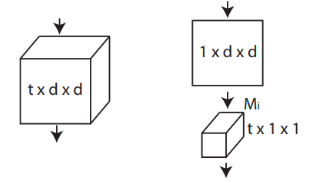
\includegraphics[width=\linewidth]{assets/img/r2+1d.png}
        \caption{(2+1)D convolutional block. (Image courtesy \cite{r(2+1)d})}
    \end{figure}
    \item It doubles the number of nonlinearities in the network due to the additional ReLU between the 2D and 1D convolution in each block.
    \item Converting the 3D convolution into separate spatial and temporal components renders the optimization easier. This results in lower training error compared to 3D convolutional networks of the same capacity.
\end{itemize}

\subsubsection{Architecture}

\begin{figure}[H]
	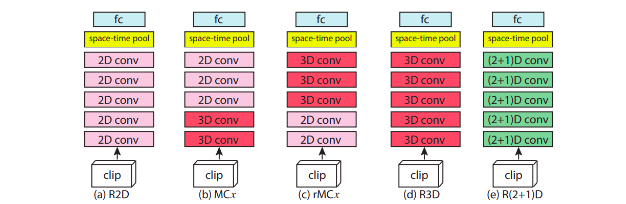
\includegraphics[width=\linewidth]{assets/img/r2+1d_arch.png}
	\caption{Residual network architectures for video classification considered in this work. (Image courtesy \cite{r(2+1)d})}
\end{figure}

\subsubsection{Conclusion}
\par R(2+1)D Architecture achieves results comparable or superior to the I3D on Sports1M, Kinetics, UCF101, and HMDB51.
This paper mostly focused on a single type of network (ResNet) and a homogenous use of our (2+1)D spatiotemporal decomposition, similar approach can be tried with different architecture. 
